\documentclass[11pt]{beamer}
\usepackage{graphicx}
\usepackage{cancel}	%para cancelar expresiones en fórmulas
\usepackage{multicol}
\usepackage{multirow}
\usepackage{amsmath}
\usepackage{float}
\usepackage{url}
\usepackage{color}
\usepackage{tablefootnote}
\usepackage[12pt]{moresize}	%más tamaños de letra
\usepackage{bm}	%bold para math

\usepackage{titlesec}
%\titleformat{\chapter}[display]
%{\normalfont\bfseries}{}{12pt}{\Huge}	%quitar header de chapter

\usepackage{siunitx}	%support for units, numbers
\sisetup{output-decimal-marker={.}, separate-uncertainty}

\usepackage{hyperref}
\hypersetup{
	colorlinks=true,
	linkcolor=blue,
	citecolor=red,
	bookmarksopen=true,
	bookmarksopenlevel=1,
	urlcolor=blue
}

\usepackage{tikz}	%%TIKZ for drawings, shapes
\usetikzlibrary{positioning}
\tikzset{
	nodo/.style={
		rectangle,
		draw,
		black,
		thick,
		rounded corners,
		node distance=1.5cm,
		inner sep=0.3cm,
		font=\large
	}
}

%%% NOMBRES DE COSAS
\renewcommand{\abstractname}{Abstract}
\renewcommand{\figurename}{Figura}
\renewcommand{\tablename}{Tabla}
\renewcommand{\contentsname}{Table of Contents}
\renewcommand{\appendixname}{Appendix}
\renewcommand{\bibname}{Referencias}
\renewcommand{\chaptername}{Chapter}

%%% COMANDOS COMUNES
\newcommand{\dif}{\text{d}}
\newcommand{\ddt}[1]{\frac{\dif #1}{\dif t}}
\newcommand{\der}[2]{\frac{\dif #1}{\dif #2}}
\newcommand{\mder}[3]{\frac{\dif^{#3}#1}{\dif #2^{#3}}}		%derivada múltiple
\newcommand{\norm}[1]{\left\| #1 \right\|}
\newcommand{\an}{($\alpha$,n) }
\newcommand{\Aliso}{\textsuperscript{27}Al }
\newcommand{\Piso}{\textsuperscript{30}P }
\newcommand{\Na}{\textsuperscript{22}Na }

%%%%%%%%%%%%%%%%%%%%%%%%%%%%%%%%%%%%%%%%%%%%%%%
\usetheme{Boadilla}
\setbeamercovered{transparent} 
\setbeamertemplate{navigation symbols}{} 
\makeatother
\setbeamertemplate{footline}{
	\leavevmode
	\hbox{
		\begin{beamercolorbox}[wd=.4\paperwidth,ht=2.25ex,dp=1ex,center]{author in head/foot}
			\usebeamerfont{author in head/foot}\insertshortauthor
		\end{beamercolorbox}
		\begin{beamercolorbox}[wd=.6\paperwidth,ht=2.25ex,dp=1ex,center]{title in head/foot}
			\usebeamerfont{title in head/foot}\insertshorttitle\hspace*{3em}
			\insertframenumber{} / \inserttotalframenumber\hspace*{1ex}
		\end{beamercolorbox}
	}
	\vskip0pt
}
\makeatletter

\author{Erik Cárdenas Mayoral}
\title{Medida de reacciones \an en CNA/HiSPANoS}
\titlegraphic{\includegraphics[scale=0.075]{us.png}} 
\institute{Máster Inter-Universitario de Física Nuclear}
\date{24/07/2023} 


\begin{document}

\begin{frame}
\titlepage
\end{frame}

%\begin{frame}
%\tableofcontents
%\end{frame}

\begin{frame}{Introducción}
	\[ ^\text{A}_\text{Z}\text{X} + ^4_2\text{He}^{2+} \longrightarrow \text{ } ^{\text{A}+3}_{\text{Z}+2}\text{Y} + \text{n}     \]
	\begin{figure}[H]
		\centering
		\includegraphics[width=0.35\textwidth]{anreaction.png}
		\caption{Ilustración de una reacción \an.}
		\label{anreaction}
	\end{figure}
\end{frame}

\begin{frame}{Relevancia de reacciones \an}
	\begin{itemize}
		\item Experimentos de partículas subterráneos: fondo de neutrones
		\item Partículas $\alpha$ de 4 a \qty{9}{\MeV}
		\item Astrofísica: procesos de síntesis de elementos
		\item Física de reactores
	\end{itemize}
	\begin{figure}[H]
		\centering
		\includegraphics[width=0.3\textwidth]{sanford.jpg}
		\caption{Experimento LUX-ZEPLIN, a \qty{1.5}{\kilo\meter} de profundidad. Fuente: \href{https://sanfordlab.org/experiment/lux-zeplin}{sanfordlab.org}}
		\label{}
	\end{figure}
\end{frame}

\begin{frame}{Objetivo del TFM}
	\begin{itemize}
		\item Medidas de \an antiguas, incompletas, y/o con grandes márgenes de error
		\item Pocas medidas de espectro de energía
		\item Dentro de la colaboración MANY, estudiar la viabilidad de medidas de \an en el CNA/HiSPANoS
		\item Para ello, medidas de TTY (activación) y espectro de energía (ToF) de \Aliso\an
	\end{itemize}
	\begin{figure}[H]
		\centering
		\includegraphics[width=0.35\textwidth]{neutronline_foto.jpg}
		\caption{Foto de la línea de neutrones HiSPANoS.}
		\label{}
	\end{figure}
\end{frame}

\begin{frame}{Montaje}
	\begin{figure}[H]
		\centering
		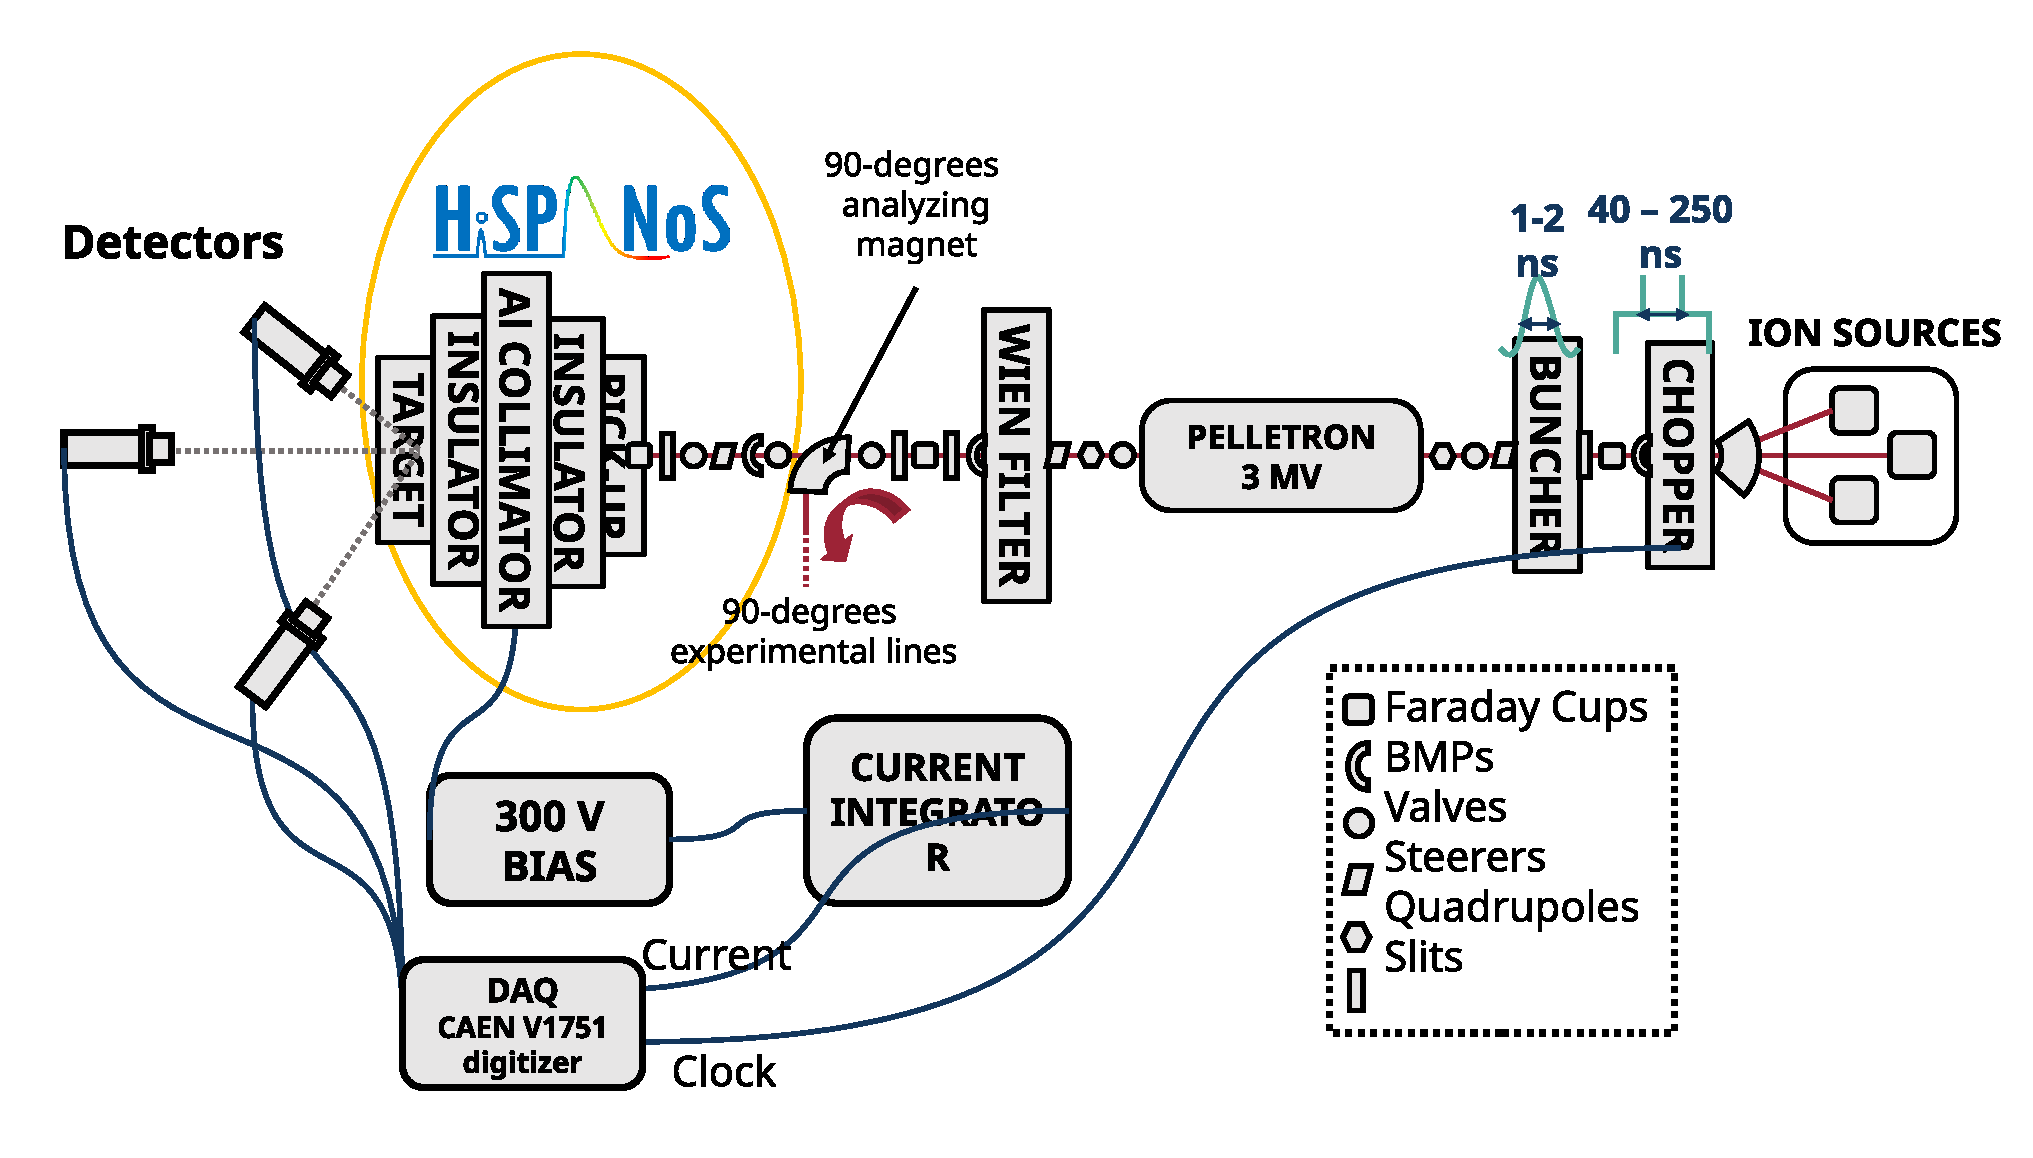
\includegraphics[width=0.75\textwidth]{tandemdiagrama.eps}
		\caption{Diagrama del acelerador Tándem del CNA.}
		\label{}
	\end{figure}
	\begin{itemize}
		\item Para $\alpha$, energía máxima de \qty{9}{\MeV}
		\item \textit{Buncher} no diseñado para partículas $\alpha$
		\item Objetivo grueso
		\item Integrador de corriente conectado al DAQ
	\end{itemize}
\end{frame}

\begin{frame}{Montaje: Detectores}
	\begin{table}[H]
		\centering
		\begin{tabular}[c]{>{\bfseries}l||c|c}
			Detector                & Distancias (\unit{\cm})& Ángulo\\ \hline
			\textbf{MONSTER}        &\num{100}, \num{200}           &\qty{60}{\degree}      \\ \hline
			\textbf{LaBr\textsubscript{3}(1)}               &\num{20} a \num{30}           &\qty{150}{\degree}     \\ \hline
			\textbf{LaBr\textsubscript{3}(2)}               &\num{20} a \num{30}           &\qty{-150}{\degree}    \\ \hline
		\end{tabular}
		\caption{Ángulos y distancias de detectores.}
		\label{distances_angles_table}
	\end{table}
	\begin{columns}
	\column{0.5\textwidth}
	LaBr\textsubscript{3}:
	\begin{itemize}
		\item Centelleador inorgánico
		\item $\gamma\longrightarrow\text{e}^-\longrightarrow$ luz centelleante
		\item Medida de eficiencia con \Na
	\end{itemize}
	\column{0.5\textwidth}
	MONSTER:
	\begin{itemize}
		\item Centelleador orgánico líquido, EJ301
		\item $\text{n}\longrightarrow\text{p}^+\longrightarrow$ luz centelleante
		\item Eficiencia obtenida de simulaciones
	\end{itemize}
	\end{columns}
\end{frame}

\begin{frame}{Montaje: Detectores - PSD}
	\begin{figure}[H]
		\centering
		\includegraphics[width=0.45\textwidth]{psd_explanation.png}
		\caption{Pulsos generados por radiación de diferentes tipos. Figura de C. Guerrero et al. \cite{guerrero2008}.}
		\label{}
	\end{figure}
	\begin{equation}
		\text{PSD} = \frac{\text{delayed}}{\text{fast}+\text{delayed}}
	\end{equation}
\end{frame}

\begin{frame}{Montaje: Detectores - PSD}
	\begin{figure}[H]
		\centering
		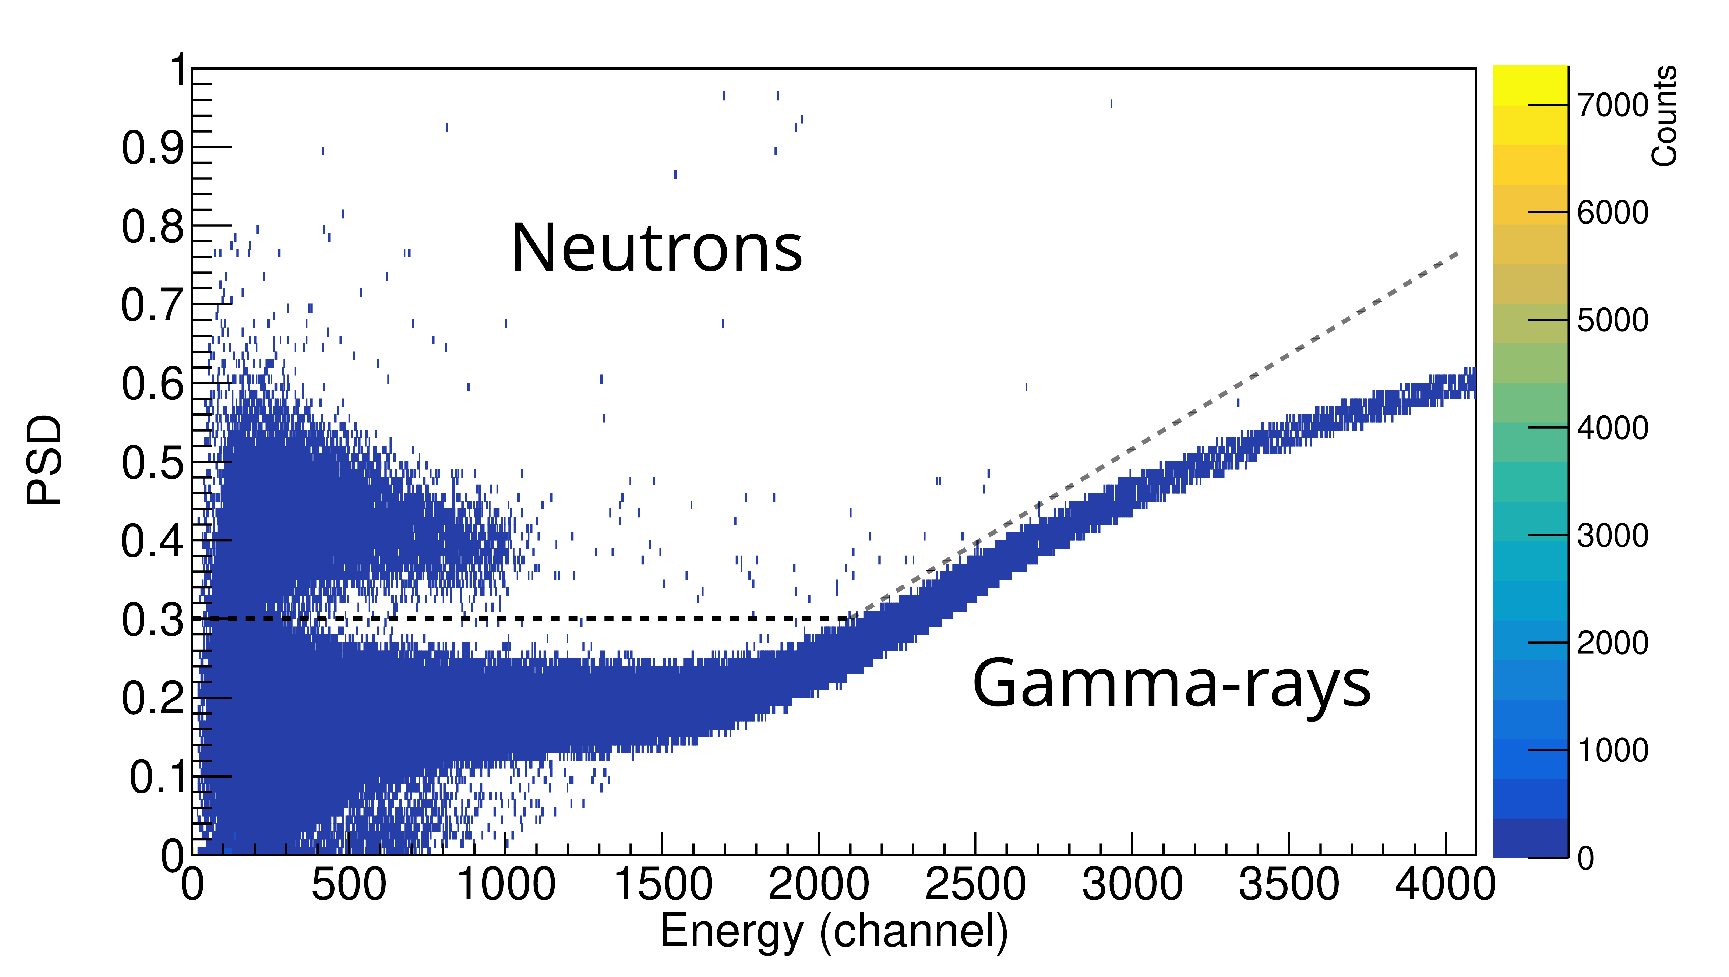
\includegraphics[width=0.85\textwidth]{example_psd.eps}
		\caption{Separación por PSD entre neutrones y rayos-$\gamma$ para una medida de MONSTER.}
		\label{}
	\end{figure}
\end{frame}



%	ACTIVACION



\begin{frame}{Medida de TTY por activación}
	\[ \text{\Aliso} + \alpha \longrightarrow \text{\Piso} + \text{n}   \]
	\centering
	$t_{1/2} = \qty{2.498(4)}{\minute}$; 
	$I_{511} = \num{1.99710(8)}$
	\begin{figure}[H]
		\centering
		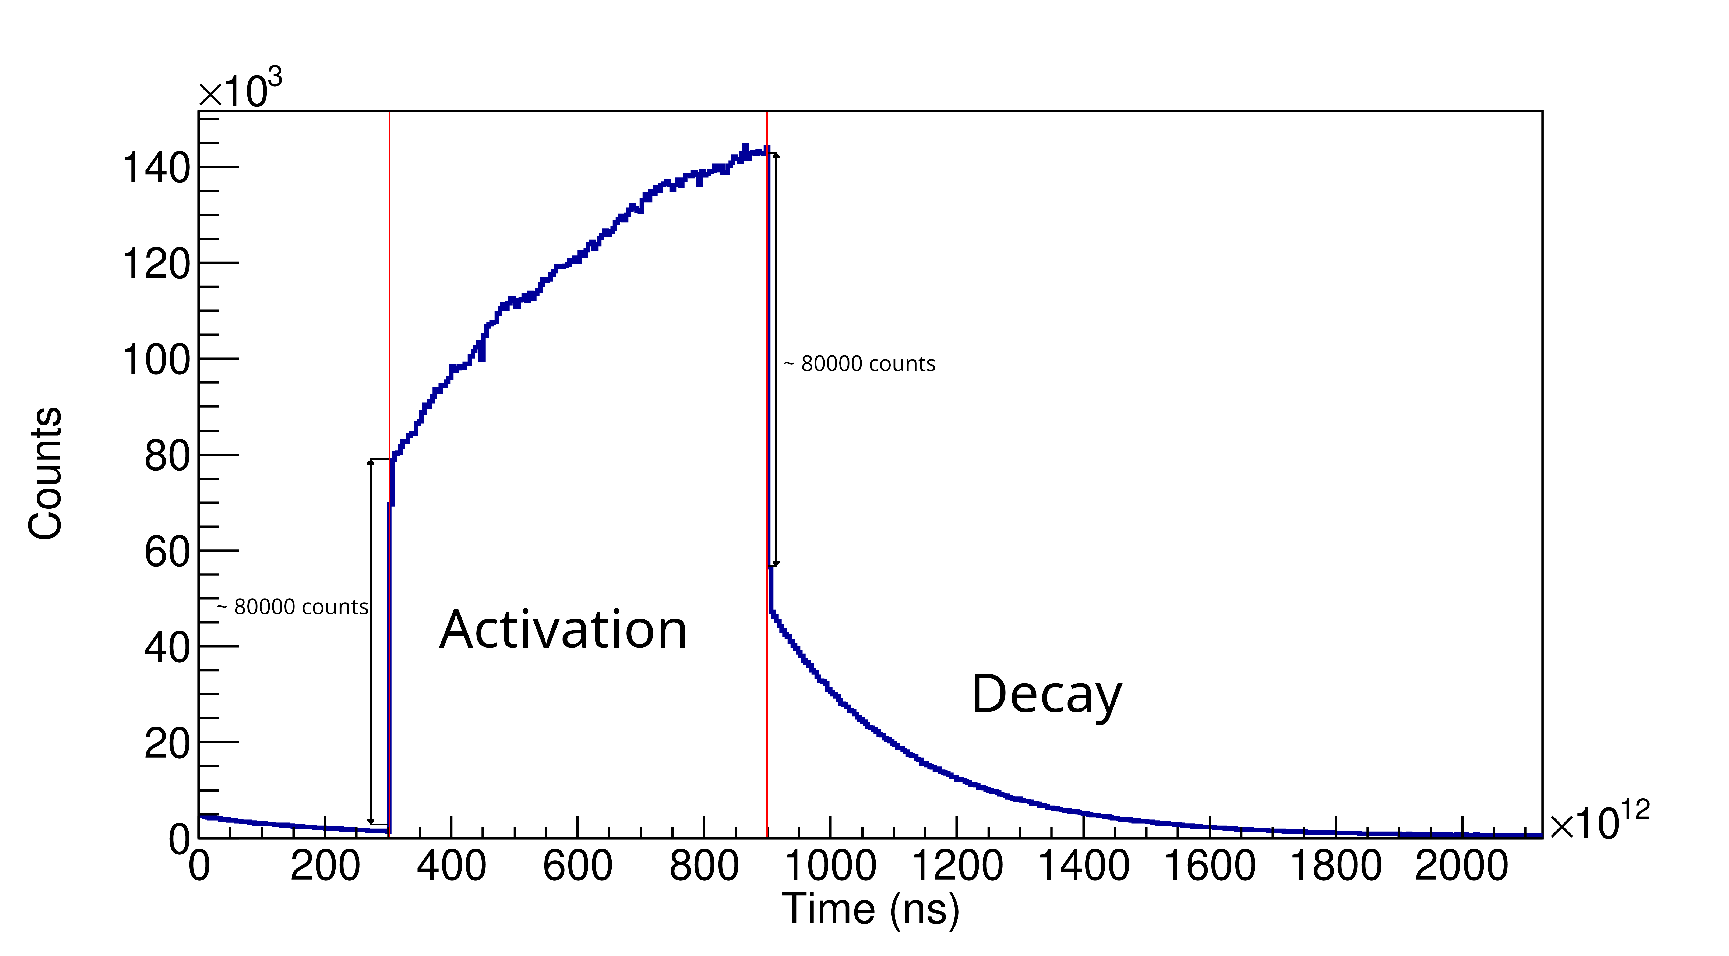
\includegraphics[width=0.80\textwidth]{example_activation_time_histogram.eps}
		\caption{Histograma de cuentas de los detectores de LaBr\textsubscript{3} frente al tiempo.}
		\label{example_activation_time_histogram}
	\end{figure}
\end{frame}

\begin{frame}{Medida de TTY por activación: CNA}
	\begin{table}[H]
		\centering
		\begin{tabular}[c]{>{\bfseries}l||c|c|c|c}
			N & Energía (\unit{\keV}) & Corriente (\unit{\nano\A}) & Irradiación (\unit{\s}) & Fecha \\ \hline
			1       &\num{5500}&\num{128}&\num{867}&22/02\\ \hline
			2       &\num{7000}&\num{101}&\num{981}&22/02\\ \hline
			3       &\num{8500}&\num{128}&\num{909}&22/02\\ \hline
			4**     &\num{8500}&\num{192}&\num{899}&23/02\\ \hline
			5       &\num{8250}&\num{193}&\num{452}&18/04\\ \hline
			6*      &\num{7000}&\num{216}&\num{466}&18/04\\ \hline
			7*      &\num{5500}&\num{151}&\num{451}&18/04\\ \hline
			8*      &\num{7500}&\num{183}&\num{448}&18/04\\ \hline
		\end{tabular}
		\caption{Medidas de activación. *: sólo carga total. **: pérdida periódica en el DAQ.}
		\label{activation_measurements_table}
	\end{table}
\end{frame}

\begin{frame}{Medida de TTY por activación: análisis}
	Número de núcleos de \Piso:
	\begin{equation}
		\ddt{N(t)} = P(t) -\lambda N(t) = P(t) - A(t)
		\label{general_diffeq}
	\end{equation}

	Definición del Thick Target Yield:
	\begin{equation}
		\text{TTY} = \frac{P(t)}{I_\alpha(t)}
	\end{equation}

	Relación entre activación y cuentas:
	\begin{equation}
		A(t) = \frac{c(t) - b(t)}{I_{511} b_{\Delta t} \varepsilon_{511}}
	\end{equation}
\end{frame}

\begin{frame}{Medida de TTY por activación: análisis \textit{decay}}
	Suponemos corriente constante:
	\begin{equation}
		\ddt{N} = P -\lambda N
	\end{equation}

	Solución:
	\begin{equation}
		N(t) = \frac{P}{\lambda} + \left(  N_0 - \frac{P}{\lambda}  \right) e^{-\lambda t}
	\end{equation}

	Tras una irradiación de duración $\Delta t$:
	\[ N\textsubscript{EOA} =N(\Delta t) = \frac{P}{\lambda} \left(1 - e^{-\lambda \Delta t} \right)\Longrightarrow A\textsubscript{EOA}=P\left(1-e^{-\lambda\Delta t}\right)\Longrightarrow \]
	\begin{equation}
		P = \frac{A\textsubscript{EOA}}{1 - e^{-\lambda \Delta t}}
	\end{equation}
\end{frame}

\begin{frame}{Medida de TTY por activación: análisis \textit{decay}}
	\begin{equation}
		\text{TTY} = \frac{P}{I_\alpha} = \frac{A_\text{EOA}}{I_\alpha \left( 1-e^{-\lambda \Delta t}  \right)} = 
		\frac{c_\text{EOA}}{I_\alpha \left( 1-e^{-\lambda \Delta t}  \right) I_{511} b_{\Delta t} \varepsilon_{511}  }
	\end{equation}
	\begin{columns}
	\column{0.65\textwidth}
	\begin{figure}[H]
		\centering
		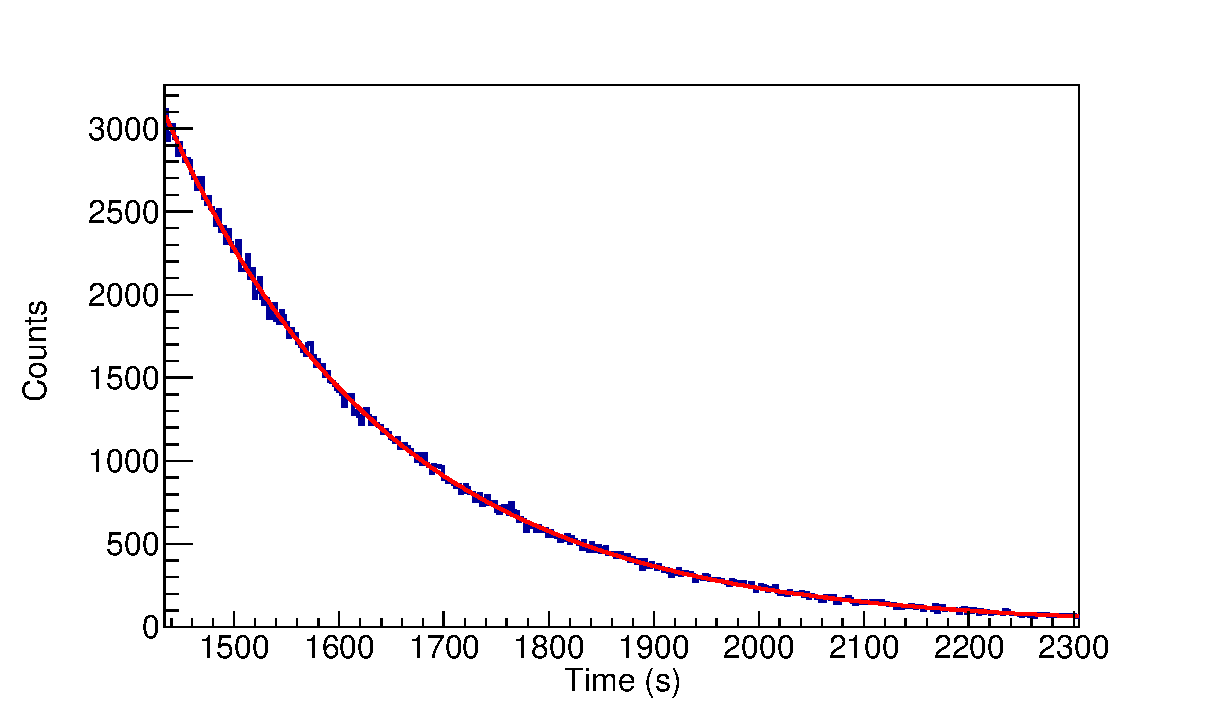
\includegraphics[width=\textwidth]{example_decay_fit.eps}
		\caption{Ajuste de decaimiento.}
		\label{decay_fit}
	\end{figure}
	\column{0.35\textwidth}
	Ajuste a ley de decaimiento más fondo:
	\begin{equation}
		c(t) = c_\text{EOA} e^{-\lambda t} + B
	\end{equation}
	\begin{itemize}
		\item Simple, rápido
		\item Estándar
		\item Considera corriente constante
	\end{itemize}
	\end{columns}
\end{frame}

\begin{frame}{Medida de TTY por activación: análisis \textit{unified}}
	Integración numérica de:
	\[\ddt{N(t)} = P(t) -\lambda N(t)\]

	\begin{figure}[H]
		\centering
		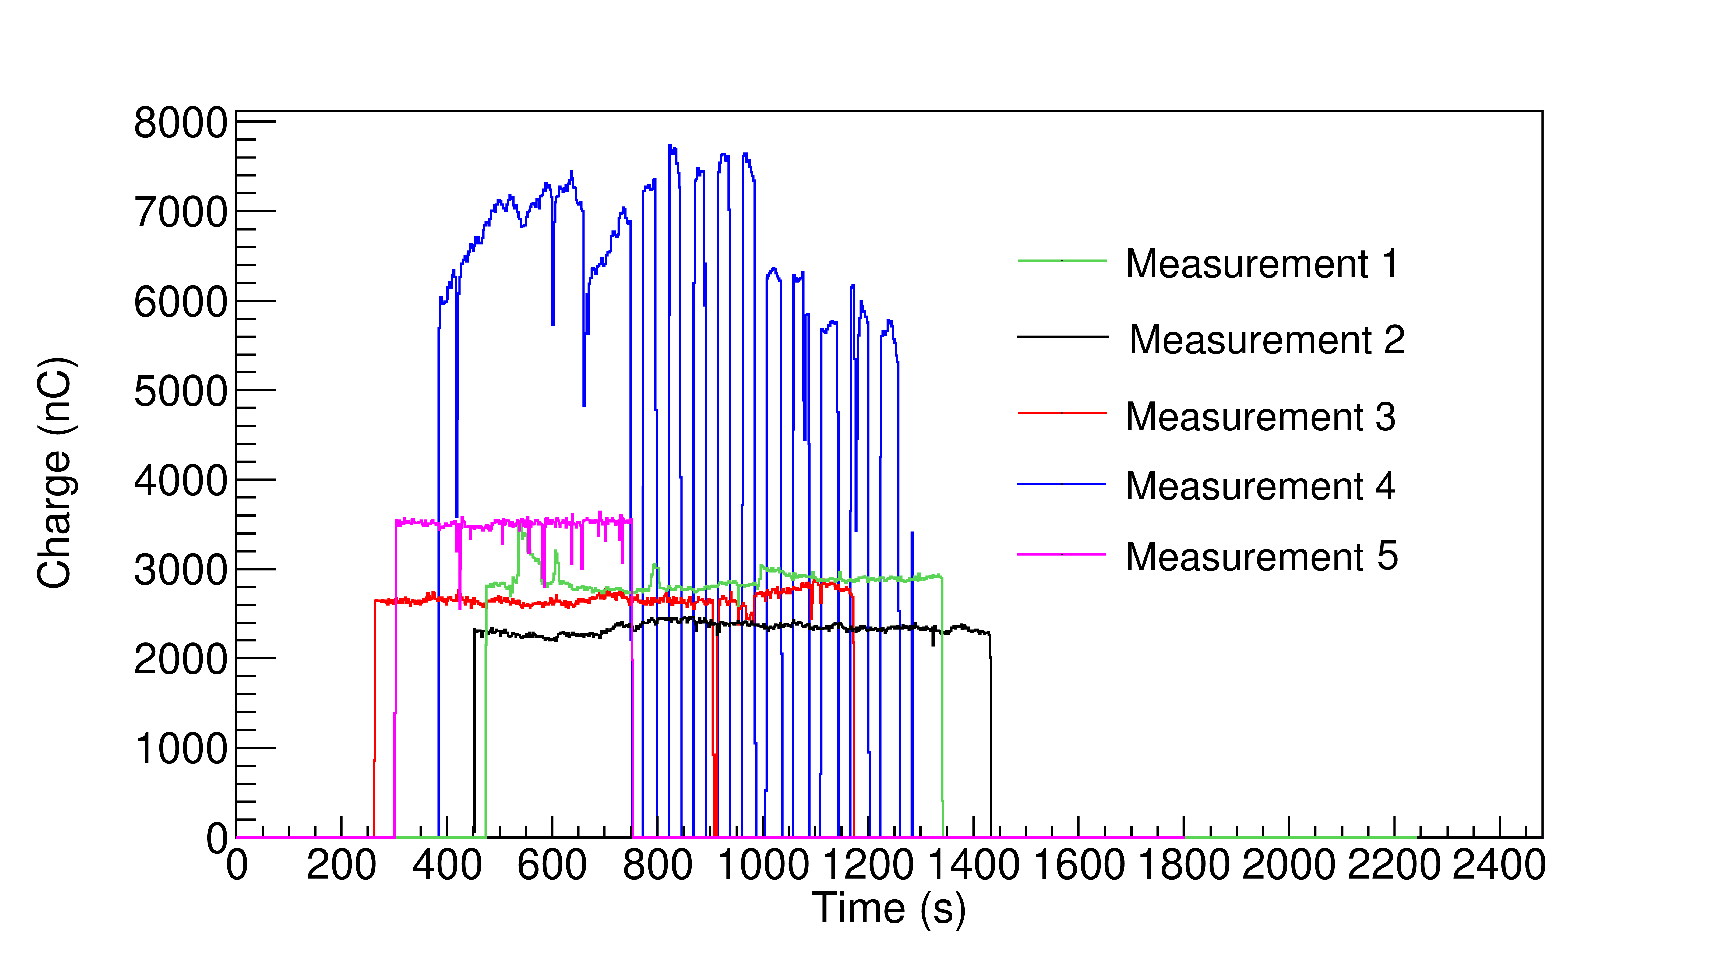
\includegraphics[width=0.80\textwidth]{current_histograms.eps}
		\caption{Superimposición de todos los histogramas de corriente.}
		\label{}
	\end{figure}
\end{frame}

\begin{frame}{Medida de TTY por activación: análisis \textit{unified}}
	Integración numérica de:
	\[\ddt{N(t)} = P(t) -\lambda N(t)\]

	Cada paso:
	\begin{equation}
		P(t) = \text{TTY}\cdot N_\alpha(t)
	\end{equation}
	\begin{equation}
		N(t+\dif t)=\frac{P(t)}{\lambda} + \left( N(t)-\frac{P(t)}{\lambda} \right) e^{-\lambda \dif t}
	\end{equation}
	\begin{equation}
		c(t) = \lambda N(t) I_{511}b_{\Delta t}\varepsilon_{511} + B
	\end{equation}

	También se tienen en cuenta el \textit{extra background} y un número de \Piso iniciales.
\end{frame}

\begin{frame}{Medida de TTY por activación: análisis \textit{unified}}
	\begin{figure}[H]
		\centering
		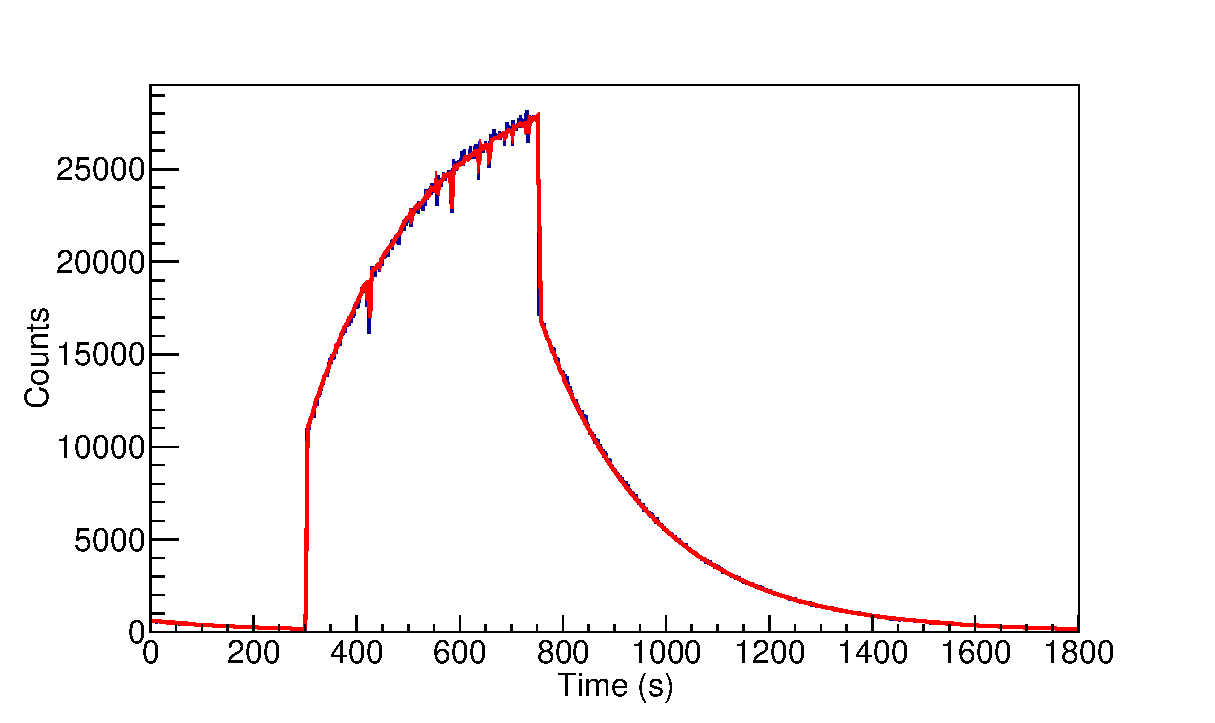
\includegraphics[width=0.7\textwidth]{example_unified_fit.eps}
		\caption{Ajuste \textit{unified}.}
		\label{unified_fit}
	\end{figure}
	\begin{itemize}
		\item No considera la corriente constante
		\item TTY aparece directamente en la función
		\item Corriente frente a tiempo no grabada para todos los datos
	\end{itemize}
\end{frame}

\begin{frame}{Medida de TTY por activación: resultados - Detectores}
	\begin{figure}[H]
		\centering
		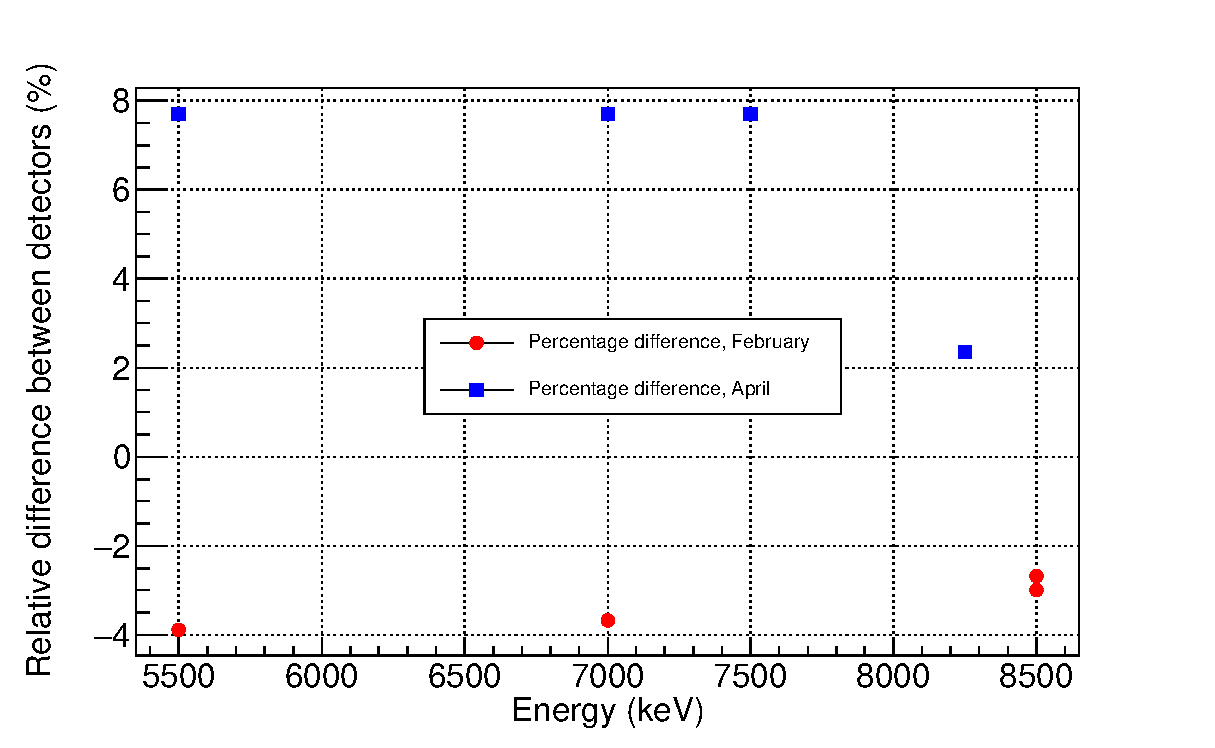
\includegraphics[width=0.75\textwidth]{decay_errors_rel_per_fixed.eps}
		\caption{Porcentaje de diferencia en resultados de TTY entre detectores.}
		\label{decay_errors_rel_per_fixed}
	\end{figure}
	Error sistemático, disminuye para energías mayores.
	Cambia de un mes a otro.
\end{frame}

\begin{frame}{Medida de TTY por activación: resultados - Métodos}
	\begin{figure}[H]
		\centering
		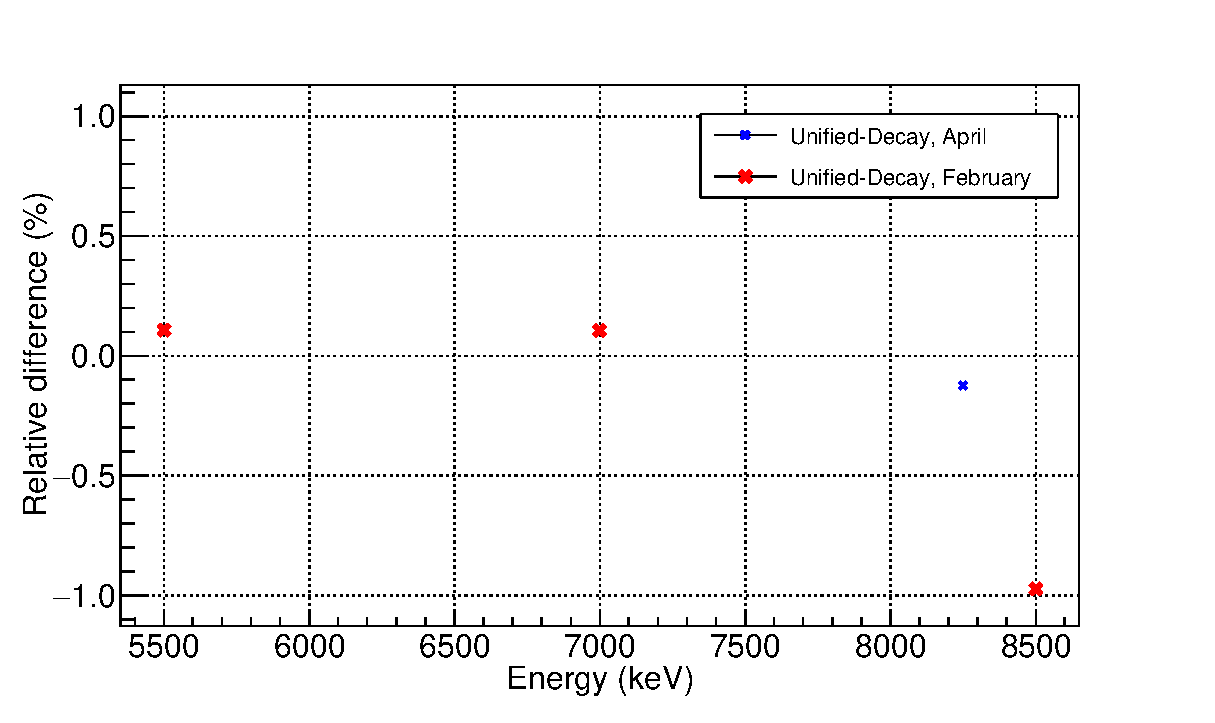
\includegraphics[width=0.80\textwidth]{activation_method_comparison.eps}
		\caption{Diferencia relativa entre diferentes métodos de ajuste.}
		\label{activation_method_comparison}
	\end{figure}
	Acuerdo dentro del \qty{1}{\percent}: el método \textit{decay} funciona bien.
	Los cambios en la intensidad del haz no son tan importantes.
\end{frame}

\begin{frame}{Medida de TTY por activación: resultados - Literatura}
	\begin{figure}[H]
		\centering
		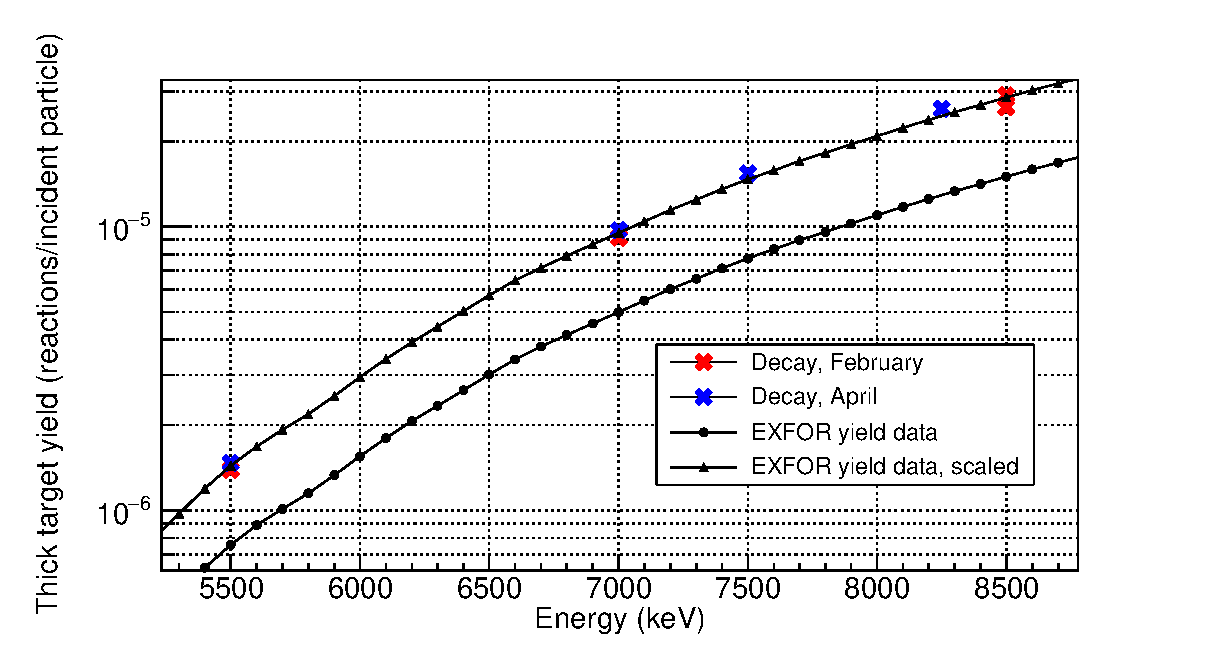
\includegraphics[width=0.80\textwidth]{activation_final_results.eps}
		\caption{Resultados obtenidos frente a G. J. H. Jacobs and H. Liskien \cite{jacobs} y a una versión escalada por \num{1.9}.}
		\label{activation_final_results}
	\end{figure}
	Gran desacuerdo, pero misma forma frente a energía.
\end{frame}

\begin{frame}{Medida de TTY por activación: resultados - Literatura}
	\begin{figure}[H]
		\centering
		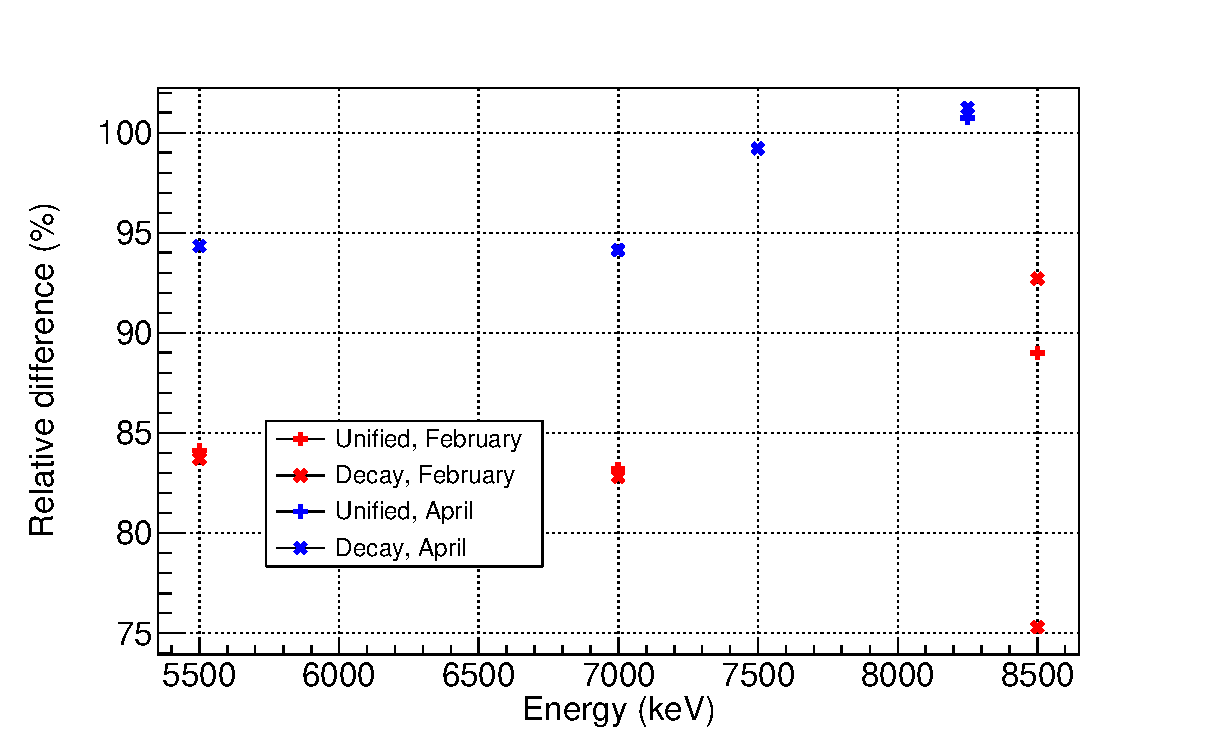
\includegraphics[width=0.80\textwidth]{activation_result_diffs.eps}
		\caption{Ratio entre valores obtenidos y G. J. H. Jacobs and H. Liskien \cite{jacobs}.}
		\label{activation_final_results}
	\end{figure}
	Factor \num{1.90(9)}. Forma reproducida en un \qty{5}{\percent}, pero con un gran error sistemático en el análisis.
\end{frame}



%	PULSADO



\begin{frame}{Espectros de energía por ToF: Principio}
	\begin{itemize}
		\item Haz pulsado
		\item \textit{Gamma flash} $L/c$ tiempo después
		\item Respuesta de neutrones con energías:
	\end{itemize}
	\begin{equation}
		E_n=\frac{1}{2} m_n \left( \frac{L}{\text{ToF}} \right)^2 = \frac{1}{2} m_n \left( \frac{L}{t_n - t_{flash} + L/c} \right)^2
	\end{equation}
	\begin{figure}[H]
		\centering
		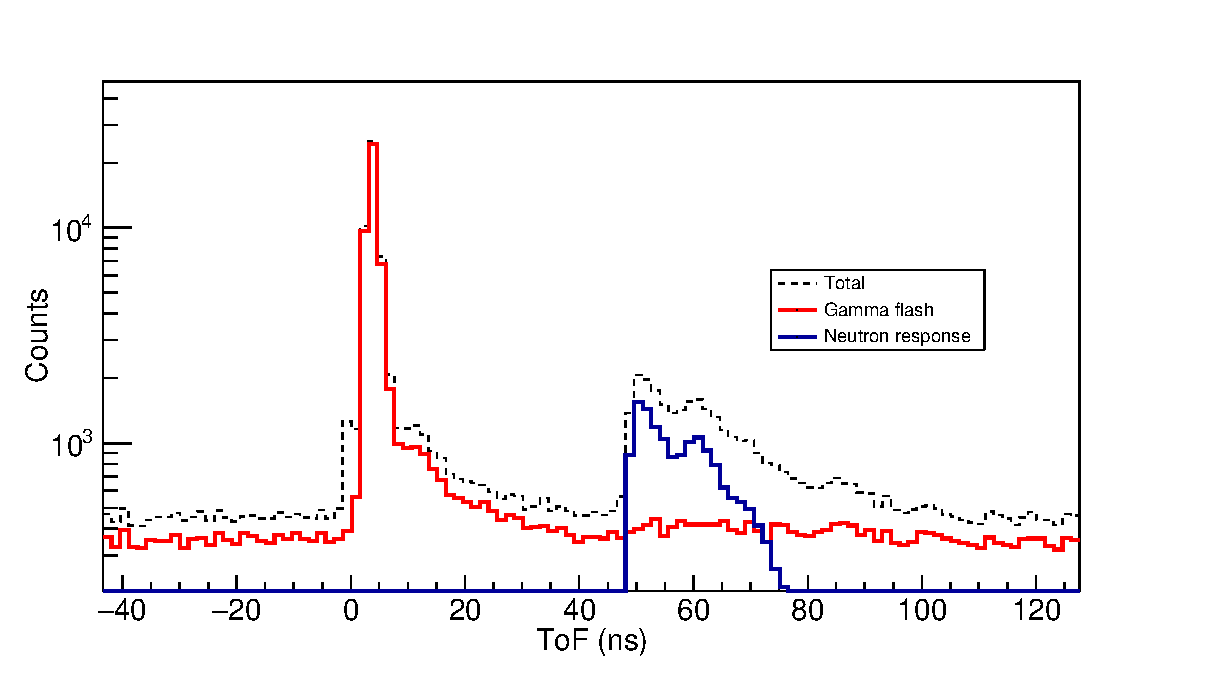
\includegraphics[width=0.70\textwidth]{separated_tof.eps}
		\caption{ToF de una medida, con el \textit{gamma flash} y la respuesta de neutrones.}
		\label{separated_tof}
	\end{figure}
\end{frame}

\begin{frame}{Espectros de energía por ToF: Medidas}
	\begin{table}[H]
	\centering
	\begin{tabular}[c]{>{\bfseries}r||c|c|c}
		N& Energía (\unit{\keV}) & Distancia (\unit{\cm}) & Fecha \\ \hline
		1&\num{5500}&\num{100.0(25)}&17 de Abril\\ \hline
		2&\num{5500}&\num{100.0(25)}&18 de Abril\\ \hline
		3&\num{7000}&\num{100.0(25)}&18 de Abril\\ \hline
		4&\num{8250}&\num{100.0(25)}&18 de Abril\\ \hline
		5&\num{8250}&\num{200.0(25)}&18 de Abril\\ \hline
	\end{tabular}
	\caption{Medidas de haz pulsado.}
	\end{table}
	\begin{figure}[H]
		\centering
		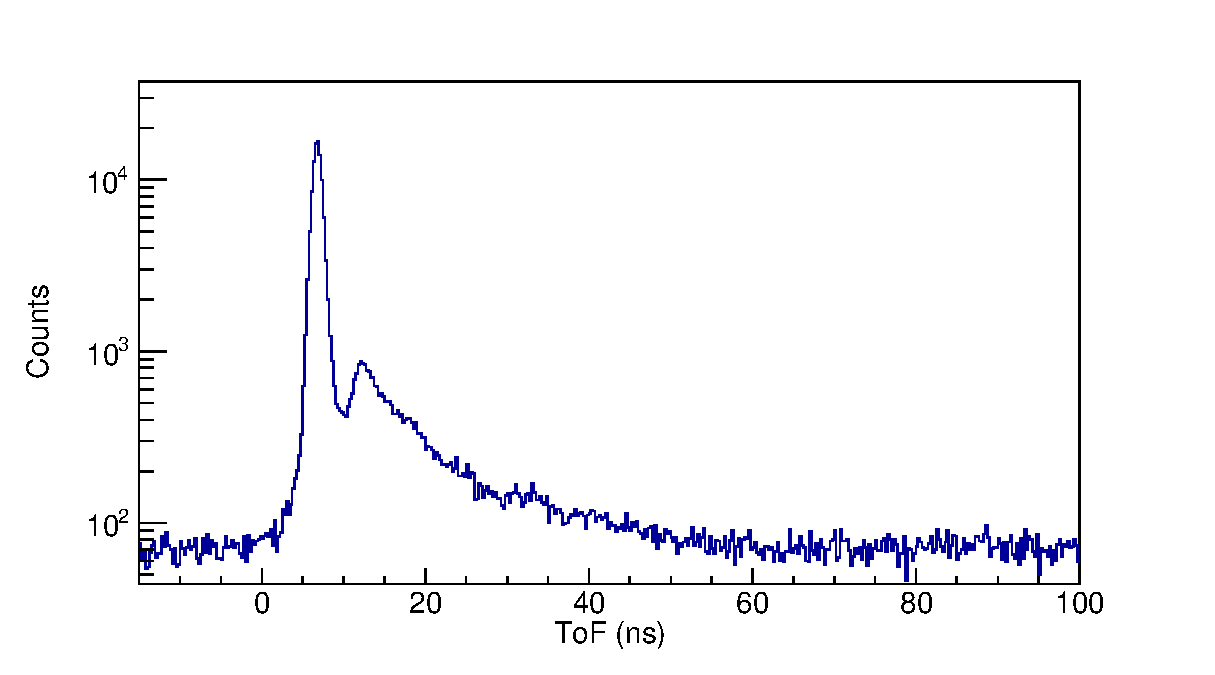
\includegraphics[width=0.50\textwidth]{uneven_gflash.eps}
		\caption{\textit{Gamma flash} de la medida 5.}
		\label{uneven_gflash}
	\end{figure}
\end{frame}

\begin{frame}{Espectros de energía por ToF: Análisis - Simple}
	\[E_n=\frac{1}{2} m_n \left( \frac{L}{\text{ToF}} \right)^2 = \frac{1}{2} m_n \left( \frac{L}{t_n - t_{flash} + L/c} \right)^2\]
	\begin{itemize}
		\item Eliminamos energías menores al \qty{15}{\percent} de eficiencia de MONSTER
		\item Corregimos por eficiencia (energética y geométrica)
		\item Resultados por $\alpha$, ángulo sólido y energía
	\end{itemize}
	\begin{figure}[H]
		\centering
		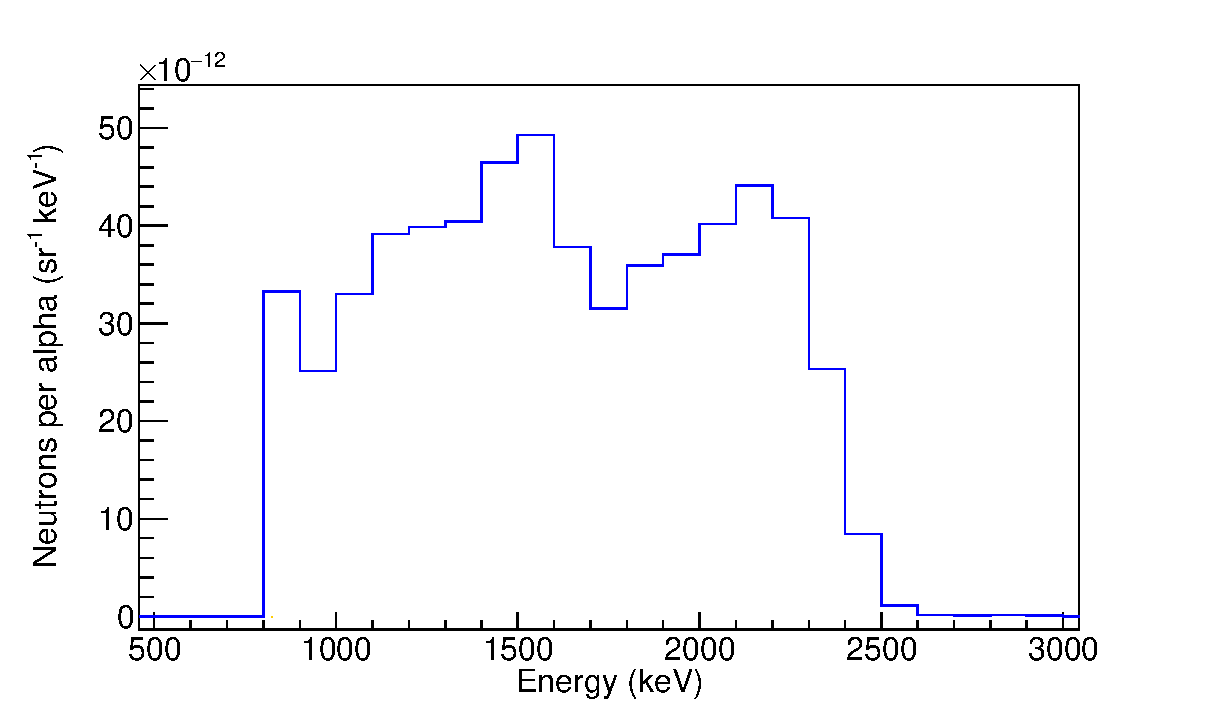
\includegraphics[width=0.60\textwidth]{pulsed_energysimple.eps}
		\caption{Espectro de energía de la medida 2.}
		\label{}
	\end{figure}
\end{frame}

\begin{frame}{Espectros de energía por ToF: Análisis - Deconvolución}
	\begin{figure}[H]
		\centering
		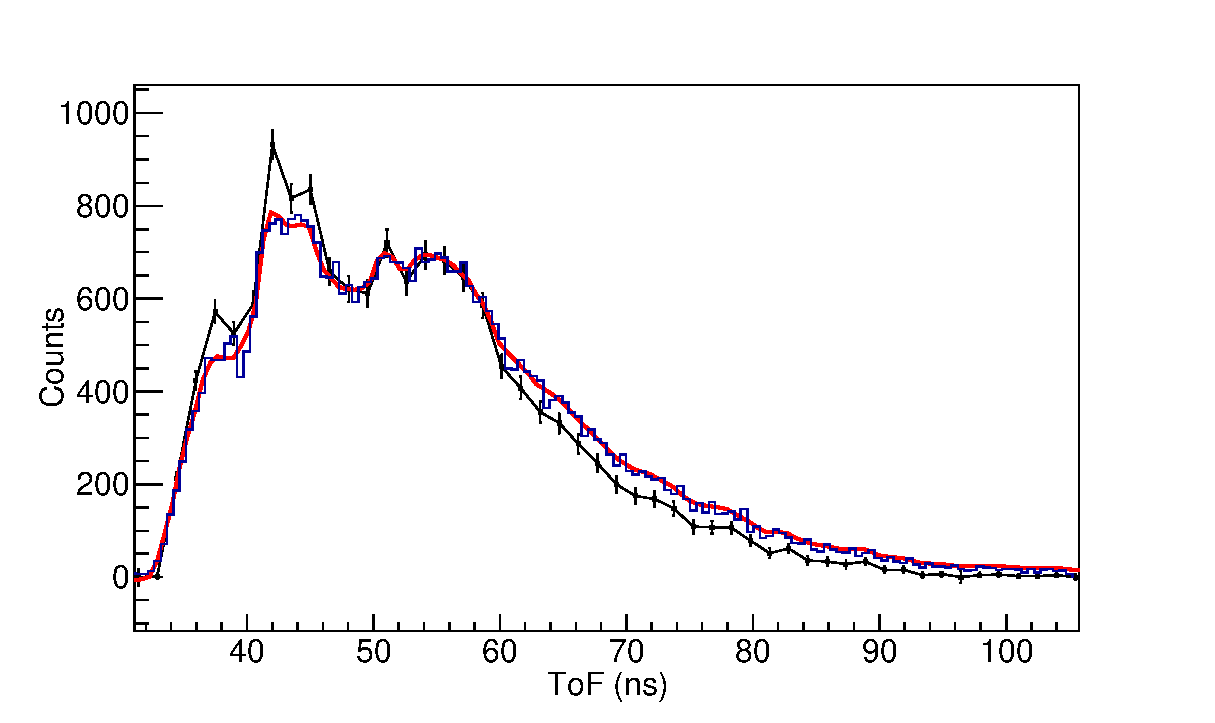
\includegraphics[width=0.70\textwidth]{pulsed_deconvolution_delta.eps}
		\caption{Deconvolución de la medida 2.}
		\label{}
	\end{figure}
	\begin{itemize}
		\item 50 parámetros representan el espectro en ToF de un $\alpha$
		\item Función usa el $\gamma$-flash para calcular la respuesta de neutrones
		\item Resultado tiene en cuenta la forma del pulso de $\alpha$
	\end{itemize}
\end{frame}

\begin{frame}{Espectros de energía por ToF: Análisis - Deconvolución}
	\begin{figure}[H]
		\centering
		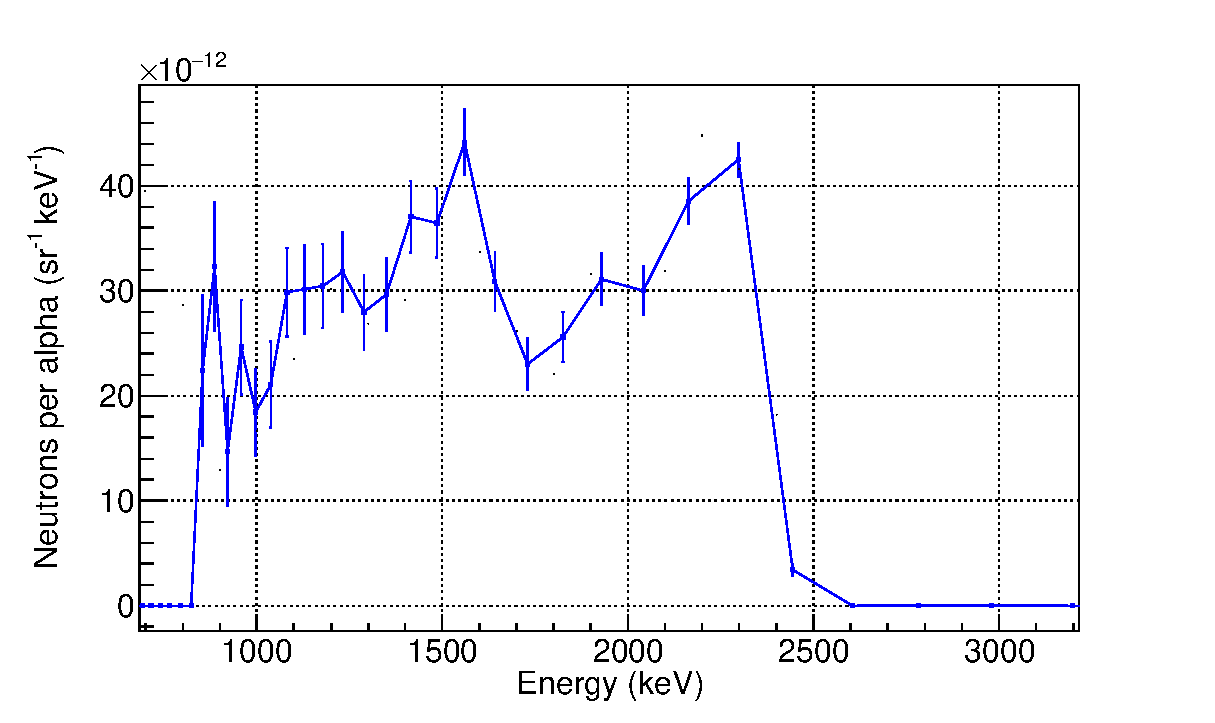
\includegraphics[width=0.70\textwidth]{pulsed_deconvolution.eps}
		\caption{Conversión de los parámetros a energía.}
		\label{}
	\end{figure}
	\begin{itemize}
		\item Parámetros repartidos equidistantes en energía
		\item Necesario ser cuidadoso al tener en cuenta la distancia en ToF
	\end{itemize}
\end{frame}

\begin{frame}{Espectros de energía por ToF: Análisis - Resultados}
	\begin{figure}[H]
		\centering
		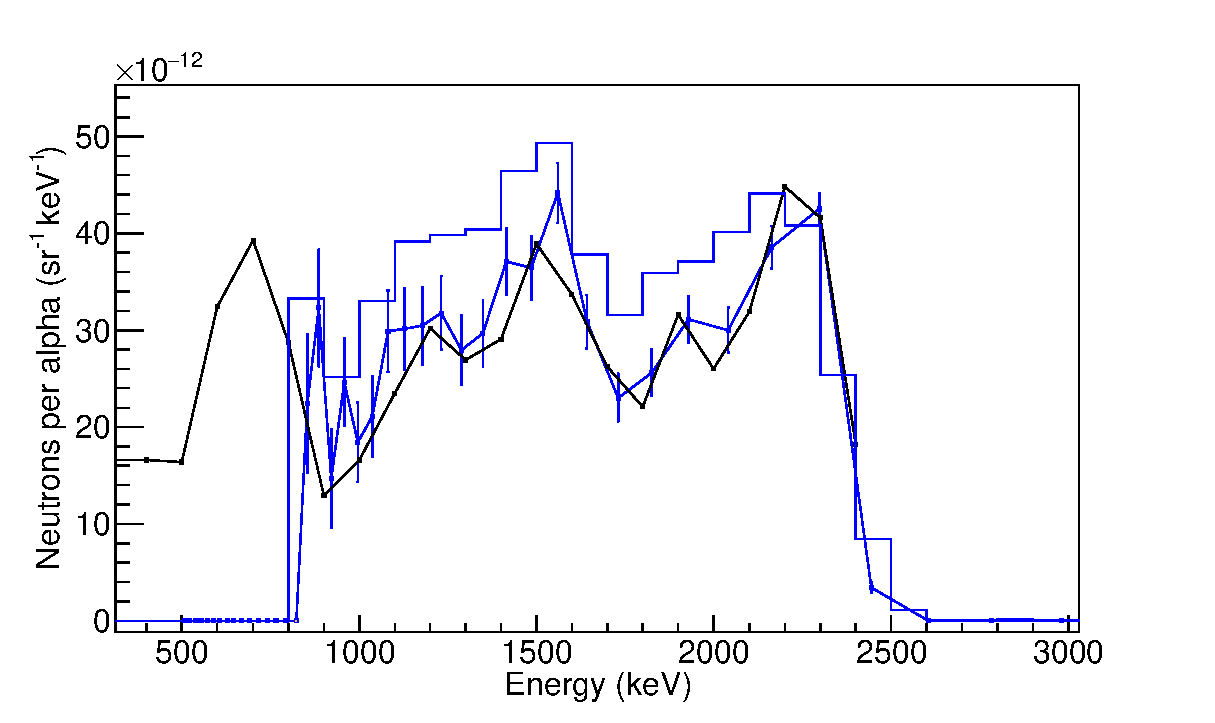
\includegraphics[width=0.70\textwidth]{pulsed_5mev.eps}
		\caption{Resultados para \qty{5.5}{\MeV}, junto con G. J. H. Jacobs and H. Liskien\cite{jacobs}.}
		\label{}
	\end{figure}
	\begin{itemize}
		\item Deconvolución mueve cuentas de bajas a altas energías: cola
		\item Mejora poco o nada la resolución
		\item Método simple sobreestima, sobretodo para bajas energías
	\end{itemize}
\end{frame}

\begin{frame}{Espectros de energía por ToF: Análisis - Resultados}
	\begin{figure}[H]
		\centering
		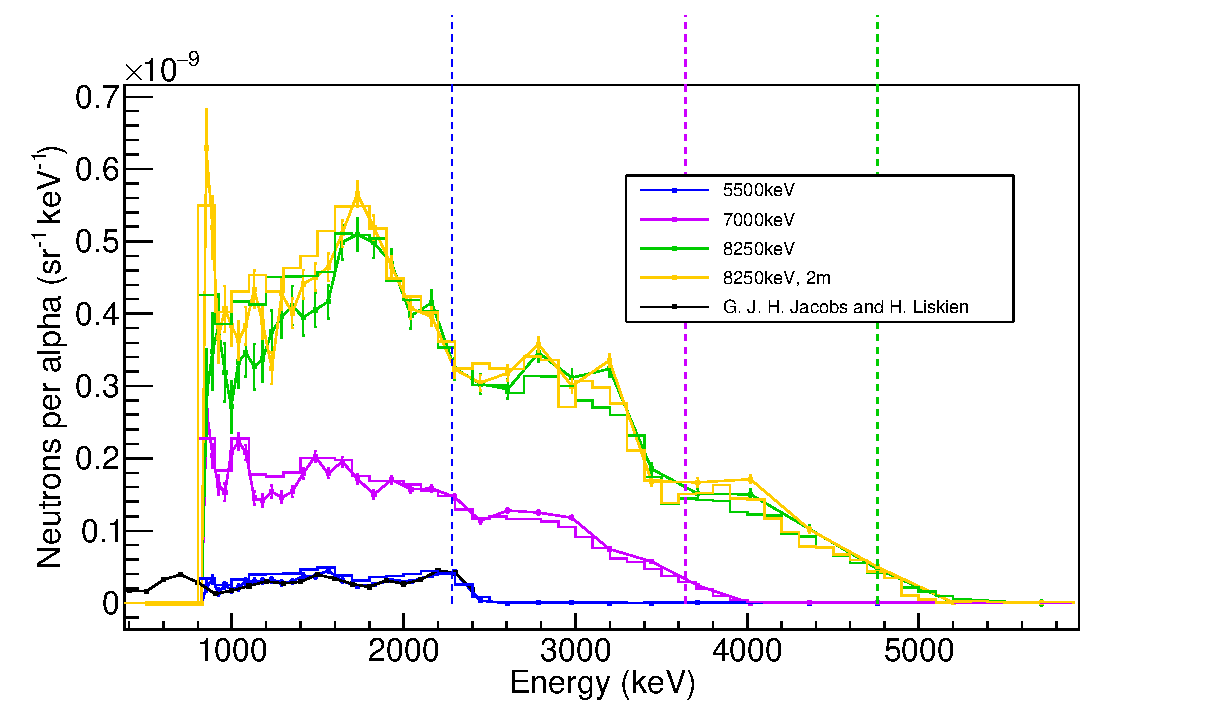
\includegraphics[width=0.70\textwidth]{pulsed_results.eps}
		\caption{Todos los resultados, por simple y por deconvolución.}
		\label{}
	\end{figure}
	\begin{itemize}
		\item Aumento con la energía de \an
		\item Poca mejora de la definición para mayor distancia
		\item Barras de error inciertas
	\end{itemize}
\end{frame}

\begin{frame}{Conclusiones}
	\begin{itemize}
		\item TTY: acuerdo entre medidas, pero gran error sistemático en análisis
		\item Método \textit{decay} suficiente: la corriente se puede tomar como constante
		\item Espectro en energía: buen acuerdo al usar una deconvolución simple
		\item Para bajas energías, usar un \textit{shadow cone} para eliminar neutrones dispersados
		\item CNA/HiSPANoS es capaz de dar medidas razonables para activación y pulsado
	\end{itemize}
\end{frame}

\begin{frame}{Referencias}
\begin{thebibliography}{5}
	\bibitem{jacobs}G. J. H. Jacobs and H. Liskien, Energy Spectra of Neutrons produced by $\alpha$ particles in thick targets of light elements, Annals of Nuclear Energy 10, 541 (1983)
%	\bibitem{hispanos}B. Fernández et al.,HiSPANoS facility and the new neutron beam line for TOF measurements at the Spanish National Accelerator Lab (CNA), 2020 J. Phys.: Conf. Ser. 1643 012033
	\bibitem{guerrero2008}C. Guerrero et al., Analysis of the BC501A neutron detector signals using the true pulse shape, Nuclear Instruments and Methods in Physics Research A 597 (2008) 212–218
%	\bibitem{astro1}F. Käppeler et al., The \textit{s} process: Nuclear physics, stellar models, and observations, Rev. Mod. Phys. 83, 157 – 193 (2011)
%	\bibitem{astro2}J. Pereira and F. Montes, Theoretical uncertainty of \an reactions relevant for the nucleosynthesis of light r-process nuclei in neutrino-driven winds, Phys. Rev. C 93, 034611 (2016)
%	\bibitem{neutron_in_an}NV.A. Kudryavtsev, P. Zakhary. B. Easeman, Neutron production in \an reactions, Nucl. Instrum. Methods Phys. Res. A 972 (2020)
%	\bibitem{MANY}N. Mont-Geli et al., miniBELEN: A modular neutron counter for \an reactions, EPJ Web of Conf., 284 (2023) 06004
	\bibitem{nucleardatasheets}M. Shamsuzzoha Basunia, Nuclear Data Sheets 111, 2331 (2010)
	\bibitem{INDC}S. S. Westerdale et al., (alpha,n) Nuclear Data Evaluations and Data Needs, Technical Report, INDC(NDS)-0836 (2022)
	\bibitem{CNA}Gómez-Camacho, J., García López, J., Guerrero, C. et al., Research facilities and highlights at the Centro Nacional de Aceleradores (CNA). Eur. Phys. J. Plus 136, 273 (2021)
%	\bibitem{labr}Alain Iltis et al., Lanthanum halide scintillators: Properties and applications, Nuclear Instruments and Methods in Physics Research Section A: Accelerators, Spectrometers, Detectors and Associated Equipment, Volume 563, Issue 2 (2006)
%	\bibitem{MONSTER}A R Garcia et al., MONSTER: a time of flight spectrometer for $\beta$-delayed neutron emission measurements, 2012 JINST 7 C05012
%	\bibitem{ej301}NEUTRON/GAMMA PSD EJ-301, EJ-309
%	\bibitem{jacobssupport1}R. Heaton et al., Neutron production from thick-target \an reactions, Nuclear Instruments and Methods A 276, 529 (1989)
%	\bibitem{jacobssupport2}J. K. Bair and J. Gomez del Campo, Neutron Yields from Alpha-Particle Bombardment, Nuclear Science and Engineering 71, 18 (1979)
%	\bibitem{CAEN}CAEN 751 Waveform Digitizer Family, CAEN SpA
%	\bibitem{ROOT}Rene Brun and Fons Rademakers, ROOT - An Object Oriented Data Analysis Framework, Proceedings AIHENP'96 Workshop, Lausanne, Sep. 1996, Nucl. Inst. \& Meth. in Phys. Res. A 389 (1997) 81-86. See also "ROOT" [software], Release 6.28/04
%	\bibitem{angeant4}E. Mendoza et al., Neutron production induced by $\alpha$-decay with Geant4, Nuclear Inst. and Methods in Physics Research, A 960 (2020) 163659
\end{thebibliography}
\end{frame}

\end{document}
